%%%%%%%%%%%%%%%%%%%%%%%%%%%%%%%%%%%%%%%%%%%%%%%%%%%
%
%  New template code for TAMU Theses and Dissertations starting Fall 2016.
%
%
%  Original Author: Sean Zachary Roberson
%  This version adapted for URS by Parasol lab.
%  Adapted from version 3.16.10, which was last updated on 9/29/2016.
%  URS adaptation last updated 1/9/2017.
%
%%%%%%%%%%%%%%%%%%%%%%%%%%%%%%%%%%%%%%%%%%%%%%%%%%%
%%%%%%%%%%%%%%%%%%%%%%%%%%%%%%%%%%%%%%%%%%%%%%%%%%%%%%%%%%%%%%%%%%%%%%
%%                           CONCLUSION
%%%%%%%%%%%%%%%%%%%%%%%%%%%%%%%%%%%%%%%%%%%%%%%%%%%%%%%%%%%%%%%%%%%%%

\chapter{CONCLUSION}

\section{Results}

In order to achieve, a full stack web application was built. The integration points from the textbook to the application consists of the five trees. Uploading the five trees into the platform is all that is required for the structures and dependencies of any given textbook to be fully understood and used.

\begin{figure}[ht]
    \centering
    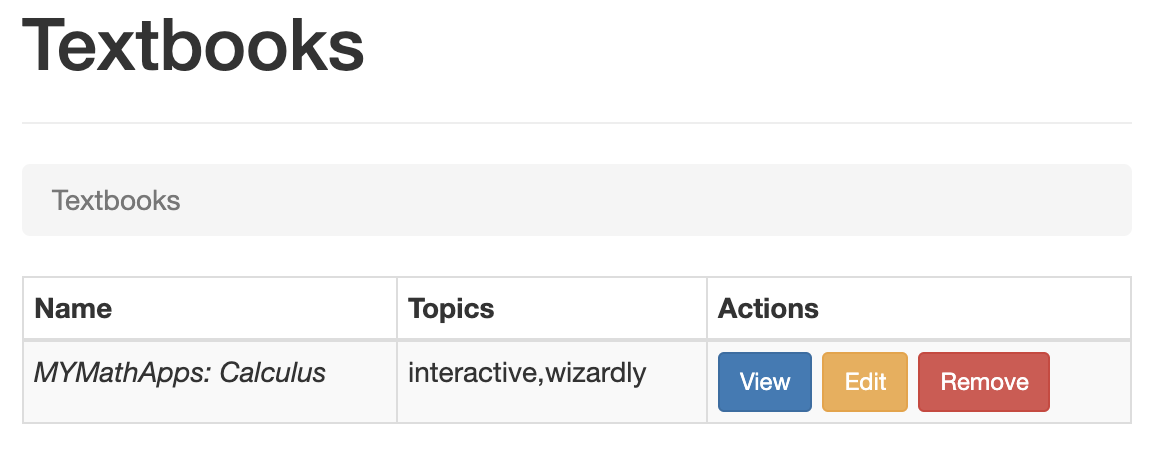
\includegraphics[scale=0.5]{textbooks.png}
    \caption[]{The selection and upload of Trees for a given textbook}
        
    \label{fig:textbooks}
\end{figure}

The next piece of the platform is the most important. It the actual piece of the platform that allows a consumer to reorder and restructure the original ordering of the textbook. It is fully interactive and draggable. Each unit and sub unit can be toggled to view more or less about units. There is also a button to toggle all units to be viewed or to collapse all units until only the independent root units are viewable.

\begin{figure}[ht]
    \centering
    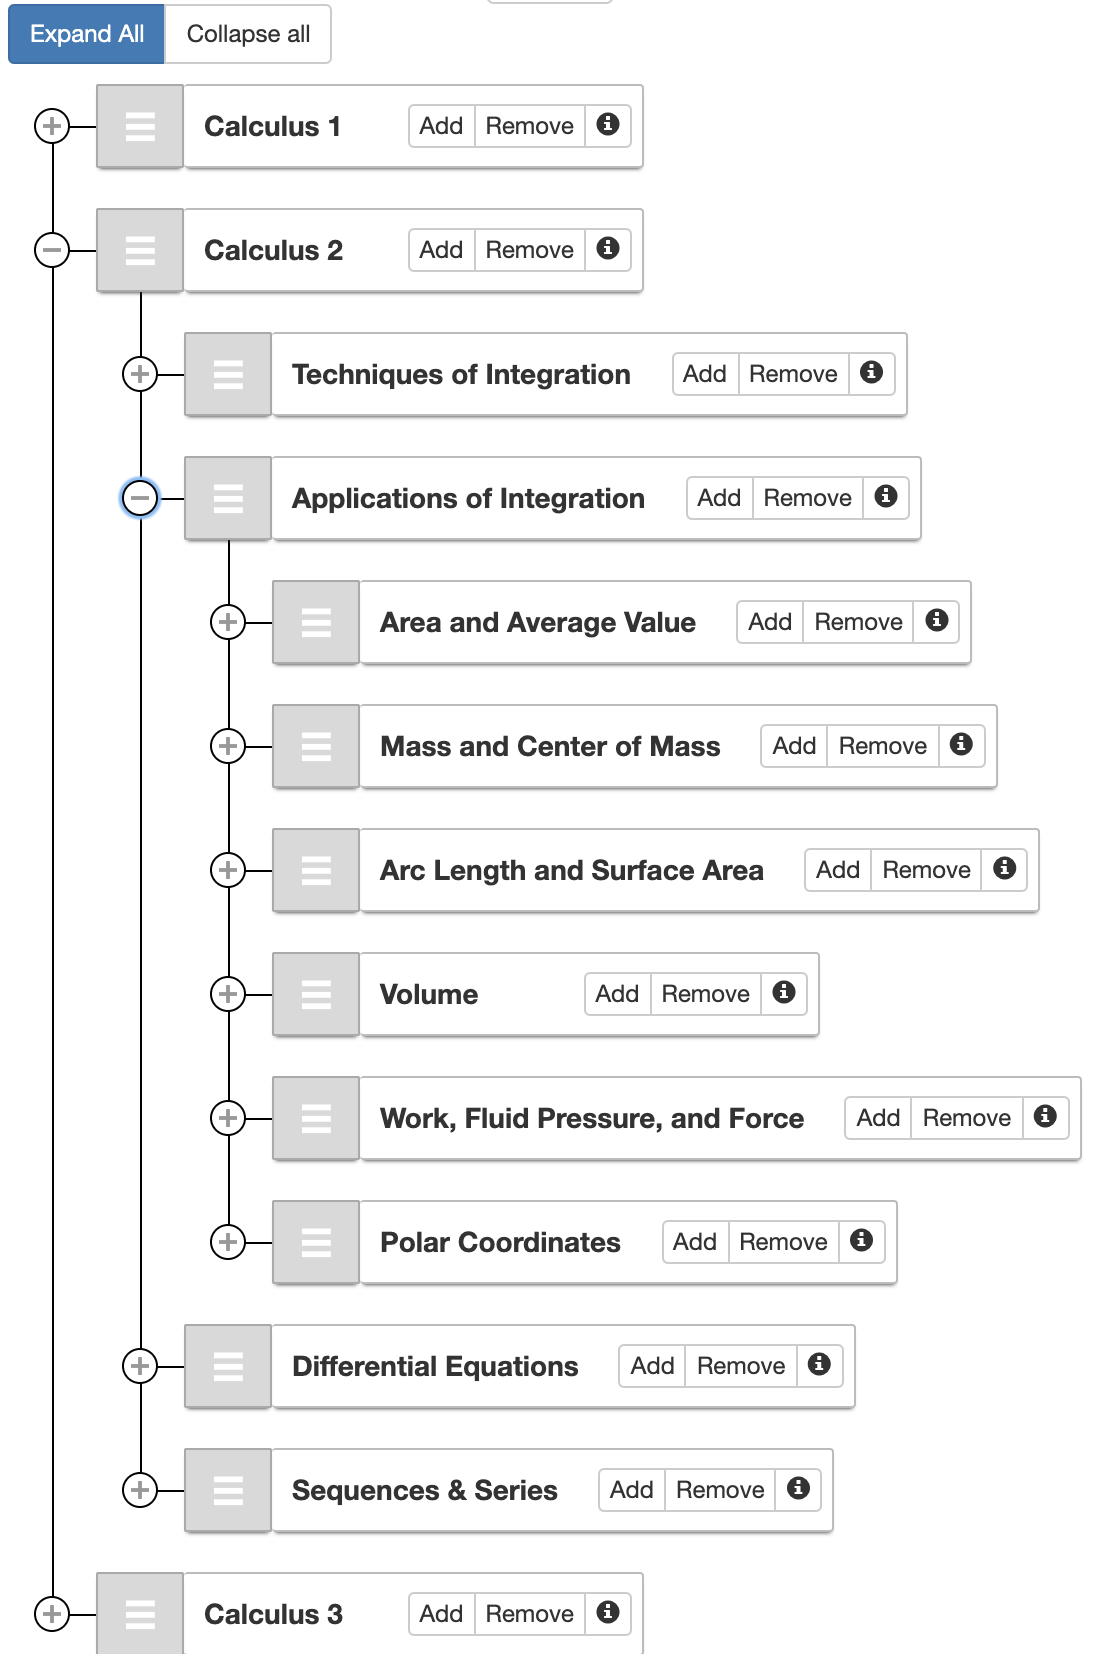
\includegraphics[scale=0.3]{nestedChapters.png}
    \caption[Unrelated topics.]{Unrelated topics. Can have any number of parents and children but do not relate to one another.}
        
    \label{fig:nestedChapters}
\end{figure}

\pagebreak

On top of being toggleable, each unit is draggable \ref{fig:chaptersMoving}. This allows for each unit to be moved to any other point in the structure of the tree or table of contents. During each of these movements, a request is sent to the server to check the and verify that all dependencies are met. If any dependency is not met, a message is then sent to the front end for it to be displayed to the user.

\begin{figure}[ht]
    \centering
    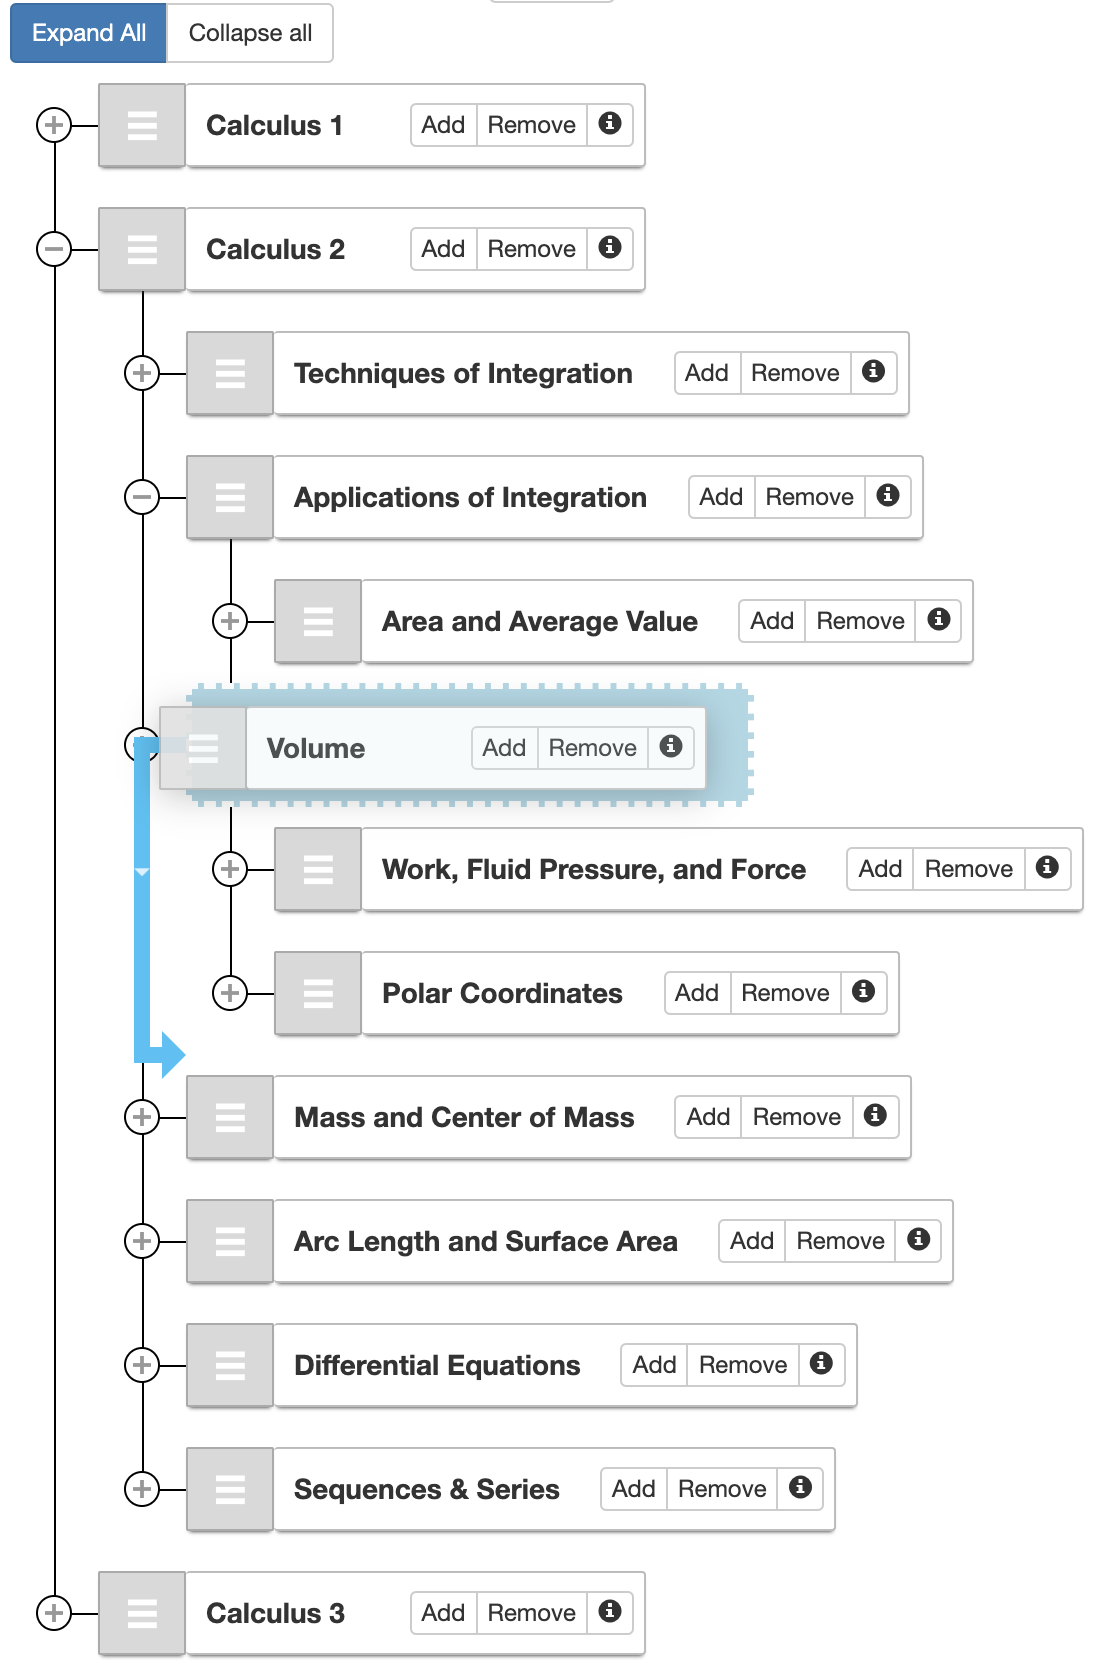
\includegraphics[scale=0.3]{chaptersMoving.png}
    \caption[Unrelated topics.]{Unrelated topics. Can have any number of parents and children but do not relate to one another.}
        
    \label{fig:chaptersMoving}
\end{figure}

\pagebreak

\section{Challenges}

One challenge encountered was the fact that the textbook was already written without this design or thoughts about the algorithm. In order to get the textbook into a place where it could be integrated with the algorithm required some slight modifications and additions. In the algorithm's current state, this is what most textbooks are required to do in order to fully integrate into the platform. This textbook used did have a similar tree structure as tree 1 (the ordering of units). With some modifications of this tree, it became the same format as required.

Another large problem encountered is related to the compounding complexity of the project. Each chapter, section and page was treated as simply as a unit. While for the purposes of dependency mapping, this group was allowable, for the use of the author of the textbook, each entity is different in both information they contain and how they may be treated for the purpose of writing the textbook.

\section{Broader Impact}

The main focus of the thesis thus far has been with a single textbook, but a broader goal is to allow any textbook to utilize this platform with the underlying algorithm. Allowing an author to use this, especially during the initial design of the textbook, will allow seamless reordering to the textbook in the event that an adopting institution or professor decides to modify the original ordering of the textbook.

\section{Future Plans}

The integration portion of the platform and textbook has not been entirely completed. There has been tweaking and modifications to the platform, the build ordering of the textbook and easily converting them into to use by the platform. A goal is to have complete integration with the textbook to the point that it can actually be tied into the build process. As a build step, any modifications can be done using the platform and then immediately carried out by producing a new version of the textbook with the appropriate modifications.
